\documentclass[]{article}
\usepackage{lmodern}
\usepackage{amssymb,amsmath}
\usepackage{ifxetex,ifluatex}
\usepackage{fixltx2e} % provides \textsubscript
\ifnum 0\ifxetex 1\fi\ifluatex 1\fi=0 % if pdftex
  \usepackage[T1]{fontenc}
  \usepackage[utf8]{inputenc}
\else % if luatex or xelatex
  \ifxetex
    \usepackage{mathspec}
    \usepackage{xltxtra,xunicode}
  \else
    \usepackage{fontspec}
  \fi
  \defaultfontfeatures{Mapping=tex-text,Scale=MatchLowercase}
  \newcommand{\euro}{€}
\fi
% use upquote if available, for straight quotes in verbatim environments
\IfFileExists{upquote.sty}{\usepackage{upquote}}{}
% use microtype if available
\IfFileExists{microtype.sty}{%
\usepackage{microtype}
\UseMicrotypeSet[protrusion]{basicmath} % disable protrusion for tt fonts
}{}
\usepackage[margin=1.5in]{geometry}
\usepackage{longtable,booktabs}
\usepackage{graphicx}
\makeatletter
\def\maxwidth{\ifdim\Gin@nat@width>\linewidth\linewidth\else\Gin@nat@width\fi}
\def\maxheight{\ifdim\Gin@nat@height>\textheight\textheight\else\Gin@nat@height\fi}
\makeatother
% Scale images if necessary, so that they will not overflow the page
% margins by default, and it is still possible to overwrite the defaults
% using explicit options in \includegraphics[width, height, ...]{}
\setkeys{Gin}{width=\maxwidth,height=\maxheight,keepaspectratio}
\ifxetex
  \usepackage[setpagesize=false, % page size defined by xetex
              unicode=false, % unicode breaks when used with xetex
              xetex]{hyperref}
\else
  \usepackage[unicode=true]{hyperref}
\fi
\hypersetup{breaklinks=true,
            bookmarks=true,
            pdfauthor={},
            pdftitle={},
            colorlinks=true,
            citecolor=blue,
            urlcolor=blue,
            linkcolor=magenta,
            pdfborder={0 0 0}}
\urlstyle{same}  % don't use monospace font for urls
\setlength{\parindent}{0pt}
\setlength{\parskip}{6pt plus 2pt minus 1pt}
\setlength{\emergencystretch}{3em}  % prevent overfull lines
\setcounter{secnumdepth}{0}

\date{}
\usepackage{lineno}
\linenumbers
\usepackage{setspace}
\doublespacing

\begin{document}

\section{Multidimensional mapping of root responses to soil
environmental cues using a luminescence-based imaging
system}\label{multidimensional-mapping-of-root-responses-to-soil-environmental-cues-using-a-luminescence-based-imaging-system}

Rubén Rellán-Álvarez\textsuperscript{1,~9}, Guillaume
Lobet\textsuperscript{2}, Heike Lindner\textsuperscript{1,~8},
Pierre-Luc Pradier\textsuperscript{1,~8,~10}, Muh-Ching
Yee\textsuperscript{1}, Jose Sebastian\textsuperscript{1}, Yu
Geng\textsuperscript{1,~7}, Charlotte Trontin\textsuperscript{1},
Therese LaRue\textsuperscript{3}, Amanda
Schrager-Lavelle\textsuperscript{4}, Cara Haney\textsuperscript{5}, Rita
Nieu\textsuperscript{6}, Julin Maloof\textsuperscript{4}, John P.
Vogel\textsuperscript{7}, José R. Dinneny\textsuperscript{1,~12}

\textsuperscript{1} Department of Plant Biology, Carnegie Institution
for Science, Stanford, CA, USA.

\textsuperscript{2} PhytoSystems, University of Liège, Liège, Belgium.

\textsuperscript{3} Department of Biology, Stanford University,
Stanford, CA, USA.

\textsuperscript{4} Department of Plant Biology, UC Davis, Davis, CA,
USA.

\textsuperscript{5} Harvard Medical School/Massachusetts General
Hospital, Department of Genetics/Department of Molecular Biology Boston,
MA, USA

\textsuperscript{6} USDA Western Regional Research Center, Albany, CA,
USA

\textsuperscript{7} DOE Joint Genome Institute, Walnut Creek, CA, USA

\textsuperscript{8} These authors contributed equally

\textsuperscript{9} Present address: Unidad de Genómica Avanzada
(Langebio), CINVESTAV, Irapuato, México.

\textsuperscript{10} Present address: Boyce Thompson Institute for Plant
Research/USDA, Ithaca, NY, USA.

\textsuperscript{11} Present address: Energy Biosciences Institute, UC,
Berkeley, CA, USA

\textsuperscript{12} Corresponding author

\textbf{Author contributions:}

RR-A: Conception, design and development of the growth and imaging
system and Arabidopsis transgenic lines; acquisition, analysis and
interpretation of data; drafting and revising the article.

GL: Development of the GLO-RIA image analysis plugin, analysis and
interpretation of data, drafting and revising the article.

HL: Acquisition of data, development of the tomato growth and imaging
setup.

P-LP: Acquisition of data, analysis and interpretation of data

MCY: Development of Arabidopsis and Brachypodium transgenic lines.

JS: Development of Brachypodium transgenic lines, acquisition and
analysis of Brachypodium data.

YG: Development of Arabidopsis transgenic lines.

CT: Acquisition and analysis of the QPCR data

TL: Acquisition and analysis of the QPCR data

AS-L: Contributed the unpublished dual-color tomato line.

CH: Contributed the unpublished \emph{Pseudomonas fluorescens} CH267-lux
strain.

RN: Contribution to the development of the Brachypodium transgenic line.

JM: Contributed the unpublished dual-color tomato line.

JPV: Contribution to the development of the Brachypodium transgenic
line.

JRD: Conception, design and development of the growth and imaging system
and Arabidopsis transgenic lines; acquisition, analysis and
interpretation of data; drafting and revising the article.

All authors read and approve the final version of the manuscript.

\subsection{Abstract}\label{abstract}

Root systems develop different root types that individually sense cues
from their local environment and integrate them with systemic signals.
This complex multi-dimensional amalgam of inputs leads to continuous
adjustment of root growth rates, direction and metabolic activity to
define a dynamic physical network. Current methods for analyzing root
biology balance physiological relevance with imaging capability. To
bridge this divide, we developed an integrated imaging system called
Growth and Luminescence Observatory for Roots (GLO-Roots) that uses
luminescence-based reporters to enable studies of root architecture and
gene expression patterns in soil-grown, light-shielded roots. We have
developed image analysis algorithms that allow the spatial integration
of soil properties such as soil moisture with root traits. We propose
GLO-Roots as a system that has great utility in both presenting
environmental stimuli to roots in ways that evoke natural adaptive
responses, and in providing tools for developing a multi-dimensional
understanding of such processes.

\subsection{Introduction}\label{introduction}

Plant roots are three-dimensional assemblies of cells that coordinately
monitor and acclimate to soil environmental change by altering
physiological and developmental processes through cell-type and
organ-specific regulatory mechanisms\textsuperscript{1,2}. Soil
comprises a complex distribution of particles of different size,
composition and physical properties, airspaces, variation in nutrient
availability and microbial diversity\textsuperscript{3,4}. These
physical, chemical and biological properties of soil can vary on spatial
scales of meters to microns, and on temporal scales ranging from
seasonal change to seconds. Root tips likely monitor this environment
through locally and systemically acting sensory
mechanisms\textsuperscript{5,6}.

The architecture of the root system determines the volume of soil where
resources can be accessed by the plant (rhizosphere). Because the
physical and chemical properties of these resources vary, their
distribution in the soil column is distinct\textsuperscript{4}. Water
and water-soluble nutrients such as nitrogen or manganese move through
the soil by bulk flow and tend to accumulate deeper in the soil profile
as a consequence of gravity\textsuperscript{7}, while other nutrients
such as phosphorus and potassium, which tightly bind to soil particles,
tend to accumulate in the upper layers of soil where decomposition of
organic matter replenishes their supply\textsuperscript{7}.
Developmental processes that affect root growth rate and direction will
influence the efficiency with which specific resources are captured from
the rhizosphere. Root systems optimized to capture one resource may be
inefficient for another.

Root architecture is under both environmental and genetic control;
plasticity in growth parameters allows the plant to adjust its form to
suit a particular soil. Lateral roots, which usually make up the
majority of the total root system, often grow at an angle divergent from
the gravity vector. This gravity set-point angle (GSA) is controlled by
auxin biosynthesis and signaling and can be regulated by developmental
age and root type\textsuperscript{8}. Recent cloning of the \emph{DRO1}
Quantitative Trait Locus (QTL) demonstrates that natural genetic
variation is a powerful tool for uncovering such control
mechanisms\textsuperscript{9}.

Specific root ideotypes (idealized phenotypes) have been proposed to be
optimal for acquisition of water and nitrogen, which are distinct from
ideotypes for low phosphorus. Based on computational modeling and field
studies, the ``steep, deep and cheap'' ideotype proposed by Lynch and
colleagues may provide advantages to the plant for capturing water and
nitrogen. This ideotype consists of highly gravitropic, vertically
oriented roots that grow deep in the soil column and develop large
amounts of aerenchyma, which reduces the overall metabolic cost of the
root system\textsuperscript{3}. Low phosphorus conditions, on the other
hand, favor roots systems that are more highly branched and shallow.
Modeling of root system variables shows that optimum architecture for
nitrogen and phosphorus uptake are not the same\textsuperscript{10} and
suggests tradeoffs that may affect the evolution of root architecture as
a population adapts to a particular environmental niche.

Clearly understanding the architecture of root systems and how
environmental conditions alter root developmental programs is important
for understanding adaptive mechanisms of plants and for identifying the
molecular-genetic basis for different response programs. Experimental
methods for studying root architecture can be divided into two general
categories that each represent compromises in either physiological
relevance or versatility.

Growth of plants in gels such as agar or gellan gum provides a
transparent support medium which allows immediate visual access to
roots. Simple devices can be used to capture macroscopic images of
roots\textsuperscript{11} or confocal microscopy can be implemented for
studying cell-scale processes. Gel-media allows exact control over the
concentration of nutrients\textsuperscript{12} or stressful
components\textsuperscript{13} and fluorescent reporters can be deployed
to track the activity of genes, proteins or metabolites. This approach
has been extensively used in the model plant Arabidopsis and has allowed
for the discovery of many fundamental processes. Root system
architecture studies and high resolution time-scale analysis of root
growth are easily performed when used in combination with automatic
time-lapse imaging\textsuperscript{14,15}. Variations of this approach
have been used in other species to study root system architecture in
three dimensions\textsuperscript{17}. Most often, in gel-based media
systems, roots are exposed to light\textsuperscript{18} while shoots are
enclosed in a high-humidity head-space that does not permit
transpiration from the leaf surface. Media is typically axenic and with
highly artificial levels and distributions of nutrients. Gas exchange
between the root and the media is limited and might lead to hypoxia or
ethylene buildup. \emph{In vitro} growth conditions are also limited in
the length of time plant growth can be supported. Typical studies
examine roots during the first 1-2 weeks after seed germination whereas
the life-cycle of Arabidopsis lasts for two months or longer, depending
on the accession. Morevover, the relevance of root architectural
phenotypes that are highly influenced by light raises concerns regarding
the importance of any loci identified using in vitro
conditions\textsuperscript{18}. Due to these limitations, studying
processes that involve whole-plant sensing of environmental cues such as
water or nutrient availability must be viewed with caution.

A less transparent but more physiologically relevant medium to study
root growth is soil. Plants are grown in soil in the field or in pots.
Root imaging can be achieved by several means, from uprooting plants
using a shovelomics pipeline\textsuperscript{\textbf{???},19} to growth
of roots in transparent pots or in rhizotrons\textsuperscript{20},
literally ``root devices'' that are constructed to allow visualization
of roots in proximity to a transparent glass or plastic plate. More
recently, the use of techniques such as X-ray micro computed tomography
has opened the possibility of \emph{in situ} characterization of root
architecture, water content and soil particles in
3-D\textsuperscript{5,21}. Such methods are limited due to their
relative cost, the volume of soil that can be imaged, the current limit
in resolution and the inability to monitor gene expression or other
molecular processes.

Roots systems have additional complexity beyond their architecture that
needs to be incorporated into our understanding of plant-environment
interactions. Primary and lateral roots exhibit different stress
response programs in Arabidopsis\textsuperscript{2} and may play
specialized roles in water and nutrient uptake. Thus, it is important to
develop methods that allow for a multidimensional characterization of
the root system that includes growth, signaling, and interactions with
other organisms.

Based on these considerations we have developed a new root imaging
platform, Growth and Luminescence Observatory for Roots (GLO-Roots),
which allows root architecture and gene expression to be studied in
soil-grown plants. GLO-Roots is an integrated system composed of custom
growth vessels, luminescent reporters and imaging systems. We use
rhizotrons that have soil volumes equivalent to small pots and support
growth of Arabidopsis from germination to senescence. To visualize
roots, we designed plant-codon optimized luciferase reporters that emit
light of different wavelengths. To visualize reporter expression, plants
are watered with a dilute luciferin solution and imaged afterwards. We
have designed a custom luminescence imaging system that automatically
captures images of rhizotrons held vertically. The signal from each
reporter is distinguished using band-pass filters held in a motorized
filter wheel, which enables automated acquisition of images from plants
expressing both structural and environmentally and developmentally
responsive reporters. We have also developed GLO-RIA (GLO-Roots Image
Analysis) software that allows for automated determination of root
system area, convex hull, depth, width and directionality, which
quantifies the angle of root segments with respect to gravity. GLO-RIA
is also able to relate root system parameters to local root-associated
variables such as reporter expression intensity or soil-moisture
content.

Overall GLO-Roots has great utility in presenting environmental stimuli
to roots in physiologically relevant ways and provides tools for
characterizing responses to such stimuli at the molecular level whole
roots of adult plants over broad time scales.

\subsection{Results}\label{results}

We have developed an integrated platform for growing, imaging and
analyzing root growth that provides advances in physiological relevance
and retains the ability to visualize aspects of root biology beyond
structure.

\subsubsection{THE GLO-ROOTS PLATFORM}\label{the-glo-roots-platform}

GLO-Roots is comprised of four parts: i) growth vessels called
rhizotrons that allow plant growth and root imaging; ii) luminescent
reporters that allow various aspects of root biology to be tracked in
living plants; iii) luminescence imaging system designed to
automatically image rhizotrons; iv) GLO-RIA, an image analysis suite
designed to quantify root systems imaged using GLO-Roots.

\paragraph{Plant growth system}\label{plant-growth-system}

GLO-Roots utilizes custom designed growth vessels classically known as
rhizotrons, which hold a thin volume of soil between two sheets of
polycarbonate plastic. Acrylic spacers provide a 2-mm space in which
standard peat-based potting mix is added. Black vinyl sheets protect
roots from light and rubber U-channels clamp the rhizotron materials
together. Plastic racks hold the rhizotrons vertically and further
protect the roots from light. Rhizotrons and rack are placed in a black
tub and about 2 cm of water are added to the bottom to maintain moisture
in the rhizotrons during plant growth. The volume of soil in the
rhizotrons (100 cm\textsuperscript{3}) is similar to small pots commonly
used for Arabidopsis growth and supports growth of Arabidopsis
throughout its entire life cycle (Fig 1A-C and Supplement 1).

While the 2 mm depth of the soil sheet is 20 times the average diameter
of the Arabidopsis root tip (approximately 100 microns), we wanted to
evaluate whether rhizotron-grown plants exhibited any obvious stress as
a consequence of physical constriction. We compared traits of plants
growing in vessels that hold similar volumes of soil but in different
geometric shapes. No significant differences in shoot area were observed
between the three systems (not shown). The number of lateral roots was
significantly lower in pot and cylinder-grown plants compared to
rhizotron-grown plants (Fig 1F) whereas primary root length of rhizotron
and cylinder-grown plants was similar and significantly greater than for
pot-grown plants (Fig 1G) . Thus, these data do not support the
hypothesis that rhizotron-grown plants experience physical constriction
greater than other vessels holding the same volume of soil.

We next compared root systems grown on the surface of agar or in soil.
Shoot weight and primary root length were significantly reduced for
gel-grown plants compared to rhizotron- or pot-grown plants suggesting
significant differences in the biology of plants grown under these
conditions (Fig 1H-I). To determine how soil-grown and gel-grown root
systems might differ in their biology, we utilized high-throughput
qRT-PCR to study a panel of 77 genes curated from the literature that
belong to a wide array of biological pathways including nutrient
acquisition and hormone and light response to abiotic stress. Whole
roots and shoot samples were collected at the end of the light and dark
cycles (16 hour light, 8 hours dark) from plants grown in rhizotrons,
pots, and petri dishes with two different media recipes (1X MS, 1\%
sucrose or 0.25X MS, no sucrose). Principal component analysis of the
gene expression values showed a clear separation of soil and gel-grown
root systems in the first two principal components with a clear overlap
between rhizotron and pot-grown root system samples (Fig 1D).
Significant differences in genes associated with flavonoid biosynthesis
(\emph{FLAVINOL SYNTHASE1, FLS1}) and phosphorus nutrition (\emph{LOW
PHOSPHATE RESPONSE1}, \emph{LPR1, PHOSPHATE STARVATION RESPONSE1, PHR1})
were observed (Fig 1E) Flavonoids contribute to anthocyanin
biosynthesis, which are UV-protectants. Importantly, however, flavonoids
have also been implicated in the regulation of root developmental
traits\textsuperscript{22}, suggesting that light-induction of these
pathways in gel-grown roots could influence such processes. \emph{SUPER
ROOT1} (\emph{SUR1}), which promotes biosynthesis of the anti-microbial
metabolite indole-glucosinolate, was significantly associated with
soil-grown roots, suggesting the non-sterile soil environment may induce
genes associated with defense. \emph{XYLOGLUCAN
ENDOTRANSGLUCOSYLASE/HYDROLASE17} (\emph{XTH17}) and TOUCH4
(\emph{TCH4}), both of which respond to touch stimuli, were expressed
more highly in soil-grown roots consistent with the presence of physical
barriers in soil while growth in gel may present fewer obstructions.
Interestingly, shoot samples where not clearly distinguished by growth
media and, instead, time of day had a greater effect (Fig. 1E and Figure
1 Supplement 1). These data suggest root systems may be particularly
sensitive to media conditions.

\paragraph{Generation of transgenic plants expressing different
luciferases}\label{generation-of-transgenic-plants-expressing-different-luciferases}

Arabidopsis roots cannot be easily distinguished from soil using
brightfield imaging due to their thinness and translucency; thus,
reporter genes are needed to enhance the contrast between the root and
their environment. Luciferase is an ideal reporter to visualize roots:
1) unlike fluorescent reporters, luciferase does not require
high-intensity excitation light, which could influence root growth, 2)
peat-based soil exhibits no autoluminescence but does autofluoresce at
certain excitation wavelengths similar to GFP (data not shown), 3) while
GFP is very stable and thus not as suitable for imaging dynamic
transcriptional events, the luciferase enzyme is inactivated after
catabolism of luciferin, making it ideal for studying processes such as
environmental responses. A considerable number of luciferases have been
developed that emit light spanning different regions of the visible
spectrum, but their utilization has been limited to studies in animals
(Table 1).

To determine the efficacy of using luciferase to visualize roots in
soil, we codon optimized sequences of \emph{PpyRe8}, \emph{CBGRed},
\emph{LUC2}, and \emph{CBG99} for Arabidopsis expression. In addition,
nanoLUC and venus-LUC2\textsuperscript{23} ~were utilized. Constitutive
luciferase expression was driven in plants using the \emph{UBQ10} or
\emph{ACT2} promoter using vectors assembled through a Golden Gate
cloning system\textsuperscript{24}. Plants homozygous for a single locus
T-DNA insertion were evaluated for in vivo emission spectra and
luminescence intensity (Fig 2A). All the evaluated luciferases use
D-luciferin as a substrate facilitating the simultaneous imaging of
different luciferases except nanoLUC, which uses a proprietary
substrate. In general, luciferases with red-shifted emission spectra
were less intense than the green-shifted luciferases (Fig 2A). LUC2o
showed an emission maximum at 580 nm and a minor peak at 620 nm while
CBG99o lacks the minor peak.

\paragraph{GLO1: a semi-automated luminescence imaging system for
rhizotrons}\label{glo1-a-semi-automated-luminescence-imaging-system-for-rhizotrons}

Luminescence imaging systems commercially available for biomedical
research are usually optimized for imaging horizontally held specimens
or samples in microtiter plates. Placing rhizotrons in this position
would induce a gravitropic response in plants. Working with Bioimaging
Solutions (San Diego, CA) we designed and built a luminescence imaging
system optimized for rhizotron-grown plants. GLO1 (Growth and
Luminescence Observatory 1) uses two back-thinned CCD cameras (Princeton
Instruments, USA) to capture partially-overlapping images of rhizotrons
while a motorized stage automatically rotates the rhizotron to capture
images of both sides (Fig 2B). A composite image is generated from the
images of each side; Fig 2C shows that approximately half of the root
system is revealed on each side with few roots being visible on both
sides. This result suggests that the depth of soil in the rhizotron is
sufficient to block visibility of roots beyond the mid-point of the soil
sheet but not so thick that a continuous root system is difficult to
reconstruct. We tested the ability of GLO1-generated images to reveal
complete root systems by manually quantifying the number of lateral
roots in root systems of 8 different plants and testing these results
against estimates of lateral root number from images visually inspected
by 4 different persons. These comparisons revealed good correlation
((R\textsuperscript{2}= 0.974)) between actual lateral root counts and
image-based estimation, indicating GLO1-generated root images provide an
accurate representation of the in soil- root system.

Continuous addition of luciferin did not have any significant effect on
shoot weight or primary root length (Figure 2 Supplement 1). After
luciferin addition, luminescence signal could be reliably detected in
root systems for up to 10 days, depending on the developmental state of
the plant.

\paragraph{\texorpdfstring{\href{https://www.dropbox.com/s/ji41jq3276vk1n5/GLO_RIA_manual.pdf?dl=0}{GLO-RIA}:
GLO-Roots Image
Analysis}{GLO-RIA: GLO-Roots Image Analysis}}\label{glo-ria-glo-roots-image-analysis}

Current image analysis algorithms are optimized for roots that are
continuously visible, since they are designed to work with images of
roots grown in transparent media or on paper. Root systems visualized
with GLO-Roots, however, often contain breaks in the continuity of
primary and lateral root signal, which likely results from soil
particles obscuring the object. We developed a set of image analysis
algorithms that were well suited for the complex root systems which
GLO-Roots is able to capture. GLO-RIA (Growth and Luminescence
Observatory Root Image Analysis) is an ImageJ plugin that can
automatically identify the perimeter of the root system and quantify
aspects of root system geometry derived from this outline. We have also
used a \href{http://fiji.sc/Directionality}{directionality algorithm}
that utilizes a sobel filter to identify edges in an image and
quantifies the proportion of quadrants that exhibit a bias in angle of
such edges with respect to the axes of the image. Similar algorithms
have been used to quantify dynamic changes in the plant
cytoskeleton\textsuperscript{25}. Directionality measurements can
rapidly capture lateral root angles at the whole root system level
without the need to define individual roots.

\subsubsection{Continuous imaging of root
growth}\label{continuous-imaging-of-root-growth}

The size of our rhizotrons enables undisturbed root system development
(before roots reach the sides or the bottom of the rhizotron) for about
21-23 days for the Col-0 accession growing under long day conditions;
however root traits besides width and depth can continue to be observed
until senescence of the plant. An example of a time series spanning 11
to 21 days after sowing (DAS) of Col-0 roots expressing
\emph{ProUBQ10:LUC2o} is shown in Fig 3A and
\href{https://www.dropbox.com/s/sxjc04o0yj2faif/Video_1.avi?dl=0}{Video
1} with a color-coded time projection shown in Fig 3B. Directionality
analysis (Fig 3C) shows a progressive change in root system angles from
0 º (vertical) to 45 º as lateral roots take over as the predominant
root type. Figure 3D shows the evolution over time of several root
traits that can be automatically captured by GLO-RIA (depth, width,
area) and others that can be manually quantified (primary root growth
rate or number of lateral roots per primary root length.

\subsubsection{Root system architecture of different Arabidopsis
accessions.}\label{root-system-architecture-of-different-arabidopsis-accessions.}

The study of natural variation for root system architecture and root
traits is a powerful approach for understanding adaptive strategies
plants use to cope with environmental change and for identifying the
genetic basis for such differences. In Arabidopsis, Quantitative Trait
Locus (QTL) and Genome-Wide Association Studies (GWAS) have led to the
identification of genes affecting root development\textsuperscript{26}.
However, traits are usually measured in seedlings less than 2 week old.
Selective pressures that affect allele frequencies in a population
likely act on genes that affect root system traits at later stages of
the plant life cycle, as well. As a proof of concept to estimate the
utility of our root imaging system to phenotype adult root system
traits, we transformed a small set of accessions with the
\emph{ProUBQ10:LUC2o} reporter and quantified RSA at 22 DAS (days after
sowing). GLO-RIA analysis of these root systems identified several root
traits that distinguish Col-0, Bay-0 and Sha (Fig 4). Bay-0 shows the
deepest and narrowest root system leading to the highest depth/width
ratio while Sha has the widest root system. Directionality analysis
revealed an abundance of steep-angle regions in the root system of Bay
while Sha showed an abundance of shallow-angled regions and Col-0 was
intermediate (Fig 4D). Broad sense heritability values for depth (96.3),
area (92.0), depth/width (97.8), width (95.7) and vertical center of
mass (95.0) were all higher than 90\%. ~

\subsubsection{GLO-Roots for Brachypodium and
Tomato}\label{glo-roots-for-brachypodium-and-tomato}

To examine the general applicability of the GLO-Roots system for other
species we introduced LUC2o-expressing reporters into the model grass
\emph{Brachypodium distachyon} and the crop plant \emph{Lycopersicon
esculentum} (tomato). Brachypodium is well suited to the GLO-Root system
because, like Arabidopsis, its small size allows mature root systems to
be studied in relatively small soil volumes\textsuperscript{27,28}.
\emph{LUC2o} driven by the \emph{ZmUb1} promoter was introduced into
Brachypodium using the pANIC vector\textsuperscript{29}. Brachypodium
roots showed a distinct architecture from Arabidopsis marked by prolific
development of secondary and tertiary lateral roots (Fig 5A). This is
consistent with other studies that show that Brachypodium has a typical
grass root system\textsuperscript{28}. After 26-28 days of growth,
shoot-derived crown roots initiated and took over as the predominant
part of the root system (not shown). Comparison of root system
development in rhizotrons with gel-based media showed that primary and
lateral root growth is more extensive in soil (Fig 5B). Interestingly,
previous work has suggested that auxin levels in Brachypodium roots is
supra-optimal for growth\textsuperscript{30}. Our results suggest that
gel-based systems may lead to an imbalance in hormone signaling that
causes slower growth.

Tomato plants were transformed with \emph{Pro35S:PPyRE8o} and
\emph{ProeDR5rev:LUC2} reporters. The plants showed more rapid growth
than Arabidopsis or Brachypodium and required fertilizer to prevent
obvious signs of stress (reduced growth, anthocyanin accumulation). Root
systems were imaged from 14 DAS plants. Roots showed less branching than
for Arabidopsis but showed many presumptive lateral root primordia
marked by DR5-expression (Fig 5C-D). These results show that the
GLO-Roots method is widely applicable to study root systems of plants
and will likely be useful for studying root systems of other small to
medium sized model and crop plants.

\subsubsection{Spectrally distinct luciferases enable characterization
of root system interactions, microbial colonization and gene expression
patterns.}\label{spectrally-distinct-luciferases-enable-characterization-of-root-system-interactions-microbial-colonization-and-gene-expression-patterns.}

Although root system architecture is usually studied in isolated plants,
this is rarely the case in nature where plants compete for soil
resources through root-root interactions. Recent work in this area has
suggested that roots from the same cultivar can grow without competition
while roots from different cultivars avoid each
other\textsuperscript{31}. One of the major challenges in such studies
is the ability to distinguish two overlapping root systems. We took
advantage of our ability to constitutively express two spectrally
different luciferases and imaged the overlapping root systems of two
Col-0 plants (one expressing \emph{ProUBQ10:LUC2o} and the other
\emph{ProACT2:PPy RE8o}) or one Col-0 plant (expressing
\emph{ProACT2:PPy RE8o}) and one Sha plant (expressing
\emph{ProUBQ10:LUC2o}). Images were captured using unfiltered light and
a custom (76.5 mm diameter) band-pass filter (415 nm - 485 nm), which
captured light emitted predominantly by LUC2o. By overlaying the images,
we were able to distinguish the two overlapping root systems (Figure 6
Supplement 1). We compared root traits of plants grown together or in
isolation but could not observe any significant differences between
treatments. This was also observed when Col-0 was grown with the Sha
accession. Further studies are warranted, however, as environmental
conditions where resources are limited may lead to more competition.

The GLO-Roots system uses non-sterile growth conditions, which allows
complex biotic interactions that may affect responses to the
environment. Bacteria themselves can be engineered to express
luminescent reporters through integration of the LUX operon, which
results in luminescence in the blue region of the spectrum and is thus
compatible with the plant-expressed luciferase isoforms we have tested.
\emph{Pseudomonas fluorescens} CH267\textsuperscript{32}, a natural
Arabidopsis root commensal, was transformed with the bacterial LUX
operon and used to inoculate plants. Thirteen days after inoculation we
were able to observe bacterial luminescence colocalizing with plant
roots. \emph{P. fluorescens} did not show an obvious pattern of
colonization at the root system scale level. As a proof-of-principle
test of the multi-dimensional capabilities of the GLO-Roots system we
visualized both \emph{LUC2o} and \emph{PPyRE8o} reporters in plants and
the LUX reporter in bacteria in the same rhizotron (Figure 6).

One of the major advantages of our system is that luciferase reporters
have been commonly used to study gene expression and these resources can
potentially be utilized to study these regulatory events in soil-grown
roots. We transformed \emph{ProACT2:PpyRE8o} into two well studied LUC
reporter lines: the auxin activity reporter line
\emph{ProDR5:LUC+}\textsuperscript{33} (Figure 7A) and the ROS activity
reporter \emph{ProZAT12:LUC}\textsuperscript{34} (Figure 7B). We
implemented in GLO-RIA an algorithm that semi-automatically identifies
gene reporter signal and associates this object to the corresponding
root structure segment. These two associated variables can be tracked in
time lapse experiments. Using the \emph{ProACT2:PpyRE8o} and
\emph{ZAT12:LUC} line we tracked root-tip associated changes in growth
and reporter expression throughout the whole root system in response to
a local application of a 1 M NaCl solution over 24 hours. As shown in
\href{https://www.dropbox.com/s/11td4zmhcw8yty6/Video_2.avi?dl=0}{Video
2}, reporter activity declines rapidly at the site of salt application
while growth and ZAT12 reporter activity become induced further away at
later time points and correlates with a burst of growth in this part of
the root system (Fig 7E-F).

\subsubsection{ADAPTIVE RESPONSES TO SOIL-BASED ENVIRONMENTAL
STIMULI}\label{adaptive-responses-to-soil-based-environmental-stimuli}

\paragraph{Phosphorus availability promotes shallow root
systems}\label{phosphorus-availability-promotes-shallow-root-systems}

To examine the effects of phosphorus availability on RSA we used alumina
particles buffered with 100 µM phosphate (P) to supply this
macro-nutrient to the root. Alumina particles bind and release inorganic
phosphorus similarly to soil particles, thus providing a physiologically
relevant nutrient regime\textsuperscript{35}. Alumina particles lacking
P, which would remove P supplied by the peat-based soil, were used to
simulate a P-deficient soil. Root and shoot phenotypes of control and
P-deficient plants at 22 (FIg 8A) and 27 (Fig 8B) DAS are shown. Plants
grown in low-P soil showed a significant increase in the width-depth
ratio of the root system compared to plants grown in P-replete soil, as
determined using the automated root system area finder in GLO-RIA (Fig
8). Plants under P deficiency showed an increase in the ratio between
root-shoot area (FIgure 8C) and higher investment of resources in the
development of the root system at the expense of shoot growth (Figure
8D). Root systems of control and P-deficient plants showed no
significant differences in directionality at 22 DAS but at 27 DAS, roots
were more horizontally oriented in P-deficient plants (Figure 8E). The
observed changes in root architecture are consistent with root system
ideotypes that improve phosphorus uptake efficiency.

\paragraph{Light promotes root gravitropism through PHOTOTROPIN
signaling}\label{light-promotes-root-gravitropism-through-phototropin-signaling}

To examine the effects of light exposure on the root system, the black
shields, which normally protect the soil and roots from light, were
removed from the top half of the rhizotron 10 DAS. Using directionality
analysis we detected a significant increase in the steepness of roots
only in the light exposed region of the rhizotron, while the lower
shielded region showed no difference. (Fig 9A-B). Light can penetrate
the top layers of soil\textsuperscript{36} and it has been proposed to
have a role in directing root growth (Figure 9 supplement 1) specially
in dry soils\textsuperscript{37} trough the blue light receptor
\emph{phot1}. Root directionality was not significantly different
between light and dark-treated roots of the \emph{phot1/2} double mutant
suggesting that blue light perception is necessary for this response
(Fig 9B), which is consistent with previous
studies\textsuperscript{37,38}. These data highlight the strong effects
of light on root system architecture\textsuperscript{18}, which
GLO-Roots rhizotrons are able to mitigate.

\paragraph{Adaptive changes in root system architecture under water
deprivation.}\label{adaptive-changes-in-root-system-architecture-under-water-deprivation.}

GLO-Roots provides important advantages over gel-based systems for
studying water-deficit (WD) responses. First, shoots are exposed to the
atmosphere and vapor pressure deficit (VPD) is maintained at levels that
allow for transpiration of water from the shoot. Second, WD can be
simulated in more realistic ways than in gel. Soil in rhizotrons is
exposed to air at the top and dries basipetally (from the top-down);
drying soil increases the volume occupied by air and reduces contact of
root with liquid water, all of which are similar to changes in soil
expected in the field during WD. Finally, as peat-based soil dries, its
optical properties change, allowing moisture content to be approximated
from bright-field images. We took advantage of the change in gray-scale
pixel intensity to construct a calibration curve (Figure 10 Supplement
1) that quantitatively relates gray-scale pixel intensity to moisture
content (Fig 10A); water content can be color coded in images with
appropriate look up tables (Fig 10B). Using this approach, water content
in a rhizotron can be mapped and visualized in 2D (Fig 10C-D) In the
example shown, we can observe that a 22 DAS Bay-0 plant depleted
soil-moisture content locally around the the root system (Figure 10E).

We performed several trials to simulate WD in our growth system. Plants
were germinated, grown under control conditions then transferred to 29ºC
and standing water was removed from the container holding the rhizotrons
starting at either 9 DAS or 13 DAS. Elevated temperature combined with
water deficit is a common stress that modern crops varieties are poorly
adapted to, thus highlighting the importance of examining this combined
treatment\textsuperscript{39,40}. Plants were maintained in this WD
regime until 22 DAS when luciferin was added and the plants were imaged.
At 13 DAS, lateral roots near the soil surface are already emerged
(\href{https://www.dropbox.com/s/sxjc04o0yj2faif/Video_1.avi?dl=0}{Video
1}, Figure 3A). After 9 days of water deficit treatment, lateral roots
showed an increase in gravitropism leading to the development of a root
system that was deeper, more vertically oriented and with more tertiary
roots (Fig 11A). Roots of Bay-0 plants showed similar responses though
the extent of change was less pronounced since Bay-0 roots are normally
more vertically oriented (Fig 11B).Plants transferred at 9 DAS showed
less lateral root development in the top layer of soil (Fig 11E). At
this time point, lateral roots start to emerge
\href{https://www.dropbox.com/s/sxjc04o0yj2faif/Video_1.avi?dl=0}{Video
1} and early drought may lead to growth quiescence or senescence. We
also grew plants under WD at control temperatures or under WW conditions
at high temperature to test the effects water and temperature had on
root architecture in isolation. We observed that both conditions were
sufficient to induce a change in root directionality indicating that the
plant uses similar mechanisms to avoid heat and water-deficit associated
stresses (Figure 11 Supplement 1). We next asked which regulatory
pathways controlled the observed changes in lateral root directionality
during simulated drought. Hydrotropism is a known environmental response
that directs root growth towards wet regions of soil. MIZ1 is an
essential regulator of hydrotropism; however miz1 mutants had no
significant effect on water deficit-induced changes in root
directionality, compared to wild type (Fig 11C), indicating that this
response was distinct from hydrotropism. Auxin is an important mediator
of gravitropism and auxin treatment causes lateral roots to grow more
vertically\textsuperscript{8}. Consistent with this role for auxin,
mutant plants with loss of function in the auxin receptor TIR1, did not
show changes in the root system directionality between WW and WD
conditions (Fig 11D).

Plants transferred at 9 DAS showed less lateral root development in the
top layer of soil.(Fig 11E) At this time point, lateral roots start to
emerge (See
\href{https://www.dropbox.com/s/sxjc04o0yj2faif/Video_1.avi?dl=0}{Video
1}) and early drought may lead to growth quiescence or
senescence\textsuperscript{2}. Careful examination of roots in these
regions showed evidence of small lateral root primordia populating
parent roots (Figure 11F). After 24 h of re-watering (Figure 11G) these
lateral root primordia reinitiated growth (Figure 11H)

Time-lapse imaging of the water deficit response showed that changes in
root growth direction occurred ahead of the dry soil front
\href{https://www.dropbox.com/s/x24x1uhvc8x0ou9/Video_3.avi?dl=0}{Video
3}. Using GLO-RIA we were able correlate water moisture contents with
local orientation of the root segments. With this approach we observed
that root segments in dryer areas of rhizotron grew at steeper root
angles (Figure 12) than roots in growing in well watered regions, though
lateral root angle in wetter regions was also affected. These data
suggest that local and systemic signaling is likely involved in
redirecting lateral roots deeper during the simulated drought treatments
tested here.

\subsection{Discussion}\label{discussion}

Organisms have evolved to acclimate to environmental change through
adaptive responses. Stressful environmental conditions can elicit
tolerance mechanisms that allow the organism to bear the negative
effects of sub-optimal conditions while avoidance mechanisms provide
alternative routes for acquiring needed resources. Environmental
stresses such as phosphate deprivation or water deficit simulated in
gel-based systems typically cause a reduction in root growth, suggesting
that the plant is preserving resources to ensure survival.
Interestingly, simulation of these same stresses using the soil-based
GLO-Roots system was able to elicit changes in root growth that are
anticipated to provide a mechanism to avoid stress. These data support
the utility of GLO-Roots for characterizing environmental responses that
are difficult to characterize otherwise.

\subsubsection{GLO-Roots enables a multi-dimensional understanding of
root
biology}\label{glo-roots-enables-a-multi-dimensional-understanding-of-root-biology}

Recent studies of root systems has emphasized structural attributes as
important contributors of root system function. Indeed, studies
examining the role of genetic variants in tolerating abiotic stress have
demonstrated the importance of such characteristics. Roots, however, are
highly diverse in the biology they perform and a multi-dimensional
understanding of root systems, which incorporates differences in
signaling, metabolism and microbial association as well as structure,
may provide a clearer understanding of the degree to which
sub-functionalization of the root system plays a role in important
processes such as acclimation and efficient resource acquisition.

We have developed tools in GLO-Roots that allow for tracking multiple
aspects of soil physicochemical properties and root biology
simultaneously. Using GLO-Roots, we are able to map in 2D coordinates
soil physical properties such soil moisture together with root
architecture traits such as directionality, growth rates and gene
expression levels. All this information is aggregated in layers for each
x, y coordinate. Using GLO-RIA we integrate this multilayer information,
leveraging our ability to simultaneously and seamlessly investigate root
responses to environmental stimuli such as soil moisture content.
Luciferase isoforms that emit light at different wavelengths allow for
constitutive and regulated promoters to be studied together.
Introduction of luciferase reporters into microbes provides an
additional layer of information that provides a readout on the
association between organisms and how this might be affected by
environmental conditions. The flexibility of the GLO-Roots system may
enable additional dimensionality to our understanding of root biology.
Other physical properties such as CO\textsubscript{2} or pH mapping in
rhizotrons have already been enabled by using planar
optodes\textsuperscript{41}. It may be possible to engineer LUX-based
reporters in microbes that are responsive to extracellular metabolites,
creating microbial biosensors, and integration of such tools may enable
root-exudation and nutrition to be analyzed in soil. Split-Luciferase
reporters have been engineered that allow bi-molecular interactions to
be studied. Finally, molecular sensors analogous to FRET sensors, termed
BRET-sensors\textsuperscript{42}, may allow metabolite tracking
dynamically through the root system. With additional innovation in the
development of luciferase reporters, the GLO-Roots systems will likely
expand the repertoire of biological processes that can be studied over
an expanded range of developmental time points and environmental
conditions.

\subsubsection{Limited phosphorus availability promotes foraging in
upper-layers of
soil}\label{limited-phosphorus-availability-promotes-foraging-in-upper-layers-of-soil}

Phosphorus availability is one of the major limitations for plant growth
and an important factor influencing root
architecture\textsuperscript{43}. P is usually more abundant in the top
layers of the soil where it is bound to organic matter and clay
minerals. Modeling studies have suggested that an increase in lateral
root density and shallower root systems promote phosphorus uptake since
phosphorus diffusibility is limited in soil and this nutrient tends to
accumulate in the upper tiers of the soil column where decomposition of
organic matter replenishes the supply of P\textsuperscript{10,44}.

Experiments using in vitro grown Arabidopsis seedlings have shown that
the primary root will senesce during low-P stress while lateral root
growth is enhanced, however the total root system area is often highly
reduced. This change in root development would be expected to reduce
energy input into the root system, but provide little advantage in
absorbing additional phosphorus. Using GLO-Roots, we demonstrate that
Arabidopsis does indeed have a robust low-P response that we predict to
enhance phosphorus uptake. While root system area is not significantly
reduced, root system width-depth ratio is increased, generating a
shallower root system. Differences between in vitro and GLO-Roots root
systems may be a result of the more physiologically realistic manner in
which phosphorus is released to the root when phosphate-buffered alumina
particles are used\textsuperscript{35}.

\subsubsection{Enhanced root growth and gravitropism may constitute an
avoidance mechanism used during
drought}\label{enhanced-root-growth-and-gravitropism-may-constitute-an-avoidance-mechanism-used-during-drought}

It has been proposed that plants with steep root systems will be better
able to tap into deep water resources and thus perform better under
water deprivation. For example in rice, the IR64 paddy cultivar shows
shallow root systems in upland fields whereas Kinandang Patong, an
upland cultivar, is deeper rooting\textsuperscript{9}. Plants maintain a
number of regulatory pathways that mediate changes in physiology during
WD. Enhanced growth of root systems has been well characterized in
field-grown plants; however this has not been recapitulated in studies
of gel-grown Arabidopsis plants. Thus, it has been unclear whether
Arabidopsis simply responds to WD differently. Our results here show
that Arabidopsis does indeed maintain a classical WD response that
expands the root system and directs growth downward. Interestingly,
under our stress regime, we did not observe a significant decrease in
the relative water content of shoot tissues (Figure 11 Supplement 2),
suggesting that the changes in root architecture were sufficient to
provide access to deep water and prevent dehydration. Such changes in
root growth are likely regulated through systemic and local signaling
that involve auxin signaling but acts independently of known pathways
that control moisture-directed root growth.

\subsubsection{Perspectives and
Conclusions}\label{perspectives-and-conclusions}

Understanding plant biology requires a sophisticated understanding of
how environmental stimuli affect the form and function of plants as well
as an understanding of how physiological context informs such responses.
Environmental conditions are at least as complex as the plants they
affect. Plant roots are exposed to a variety of environmental signals
that change in time and space at very different scales that are
integrated at the whole plant system. It is an important challenge in
biology to develop methods of growing and studying plants that present
such stimuli in a manner that the plant is likely to encounter in
nature. After all, the plants we study have evolved to survive through
mechanisms that have been selected, over evolutionary time, in nature.
Use of artificial conditions must be carefully considered especially if
adaptive mechanisms are the area of focus for the study.

The study presented here shows conclusively that root biology in
soil-like media is distinct from in vitro grown plants. These
differences are not only due to media composition but likely encompass
effects from other abiotic and biotic factors as well. It will be
interesting for future studies to determine how other environmental
stimuli affect root growth using GLO-Roots and whether these responses
differ between accessions of Arabidopsis. Identification of the genetic
loci responsible for phenotypic variation in adult root phenotypes may
identify the molecular basis for adaptive variation that exists in this
species and potentially identify loci that are useful for breeding
efforts needed for the next green revolution.

\subsection{Materials and methods}\label{materials-and-methods}

\subsubsection{Growth system}\label{growth-system}

\textbf{Rhizotrons and growth system fabrication}. Rhizotrons are
composed of two sheets of 1/8" abrasion resistant polycarbonate plastic
(Makrolon AR (R)) cut to size using a water jet (AquaJet LLC, Salem,
OR), two acrylic spacers cut using a laser (Stanford Product Realization
Lab), two rubber U-channels cut to strips 30 cm long
(\href{http://www.mcmaster.com/\#catalog/121/3838/=wdre76}{McMaster Carr
part \# 8507K33}) and two sheets of black 0.030" thick polypropylene
sheets
(\href{http://www.mcmaster.com/\#catalog/121/3616/=wdrfie}{McMaster Carr
part \# 1451T21}) cut with a straight-edge razor blade. Rhizotron
designs were drafted in Adobe Illustrator (Adobe, San José, CA). The
blueprints of all the parts are provided in Supplement 1. The top edge
of each polycarbonate sheet was painted with black 270 Stiletto nail
polish (Revlon, New York, NY).

\textbf{Boxes and holders.} Rhizotrons are held vertical during plant
growth in a custom rack system composed of two sheets of 1/4" black
acrylic plastic cut with slots for eleven rhizotrons using a laser, four
3/8" PVC rods
(\href{http://www.mcmaster.com/\#98871a041/=wdrftz}{McMaster Carr part
\# 98871a041}) secured with PVC nuts
(\href{http://www.mcmaster.com/\#94806a031/=wdrgar}{McMaster Carr part
\# 94806a031}) to hold the acrylic sheets horizontal. The rack is placed
inside a 12`` x 12'' x 12" black polyethylene tank
(\href{http://www.plastic-mart.com/product/4510/7-gallon-rectangular-tank-r121212a}{Plastic
Mart part \# R121212A}).

\textbf{Rhizotron preparation} The procedure to construct a rhizotron
with soil is as follows: Two pieces of polycarbonate plastic are laid
flat on a table with the spacers inserted. Using an electric paint gun,
a fine mist of water is applied to the bare polycarbonate sheets. Then,
using a 2 mm sieve (US Standard Sieve Series Nº 10) a fine layer of
PRO-MIX(r) PGX soil (Premier Tech, Canada) is applied. Excess soil is
discarded by gently tapping the plastic against the table in a vertical
position. Water is sprayed again onto the soil, then a second layer of
Pro-MIX is applied as before. For P deficiency experiments soil
supplemented with 1 ml of 100 µM P-Alumina (control) and 0-P-Alumina (P
deficient ) was used. To prevent the soil from falling out of the bottom
opening, a 3 x 6 cm piece of nylon mesh is rolled into a 1 cm wide tube
and placed at the bottom side of the rhizotron. The spacers are removed
and replaced by clean spacers. The two faces of the rhizotron are
carefully joined together and two rubber U-channels slipped on to clamp
all pieces together. Assembled rhizotrons are placed into the rack
inside the boxes and 500 mL of water is added to the box.

\textbf{Plant growth} \emph{Arabidopsis thaliana} seeds were stratified
for 2 d at 4 ºC in Eppendorf tubes with distilled water. Seeds were
suspended in 0.1 \% agar and 5 to 10 were sown using a transfer pipette
in the rhizotron. A transparent acrylic sheet was mounted on top of the
box and sealed with tape to ensure high humidity conditions that enable
\emph{Arabidopsis} germination. Three days after sowing, the cover was
unsealed to decrease humidity and allow the seedlings to acclimate to a
dryer environment. From 3 days after sowing (DAS) to the time the first
true leaves emerged, it was critical to ensure that the top part of the
rhizotron remained humid for proper germination of the plants. Between
three and five DAS the rhizotrons were thinned leaving only the number
plants required for that experiment, typically one, except for
experiments examining root-root interactions. Unless otherwise stated,
all the experiments presented here, treatments were started 10 DAS.
Plants were grown under long day conditions (16 h light / 8 h dark)
using 20--22 ºC (day/night) and 150 µE m--1 s--1. Two types of growth
environments were used for experiments. A walk-in growth chamber with
fluorescent lightning and a growth cabinet with white LED lights.

\subsubsection{qRT-PCR analysis.}\label{qrt-pcr-analysis.}

Seeds were surface sterilized as described before\textsuperscript{2} and
grown in rhizotrons, 100 cm\textsuperscript{3} pots, or on two types of
1\% agar (Duchefa) media containing either 1x MS nutrients (Caisson) and
1\% Sucrose, (termed ms media) or ¼x MS nutrients only (termed ms25
media). Both media were buffered using 0.5 g/L MES and pH was adjusted
to 5.7 with KOH. All plants were grown together in a growth cabinet with
LED lights under long day conditions (16h day/8h night). Root and shoot
tissue was collected separately from individual plants at the end of the
day (1 hour before the lights shut off) and at the end of the night (1
hour before lights came on). Three biological replicates were collected
for each condition. RNA was extracted using the Plant RNA MiniPrepTM kit
(ZYMO Research) according to manufacturer's instructions with on-column
DNase treatment (Qiagen). cDNA was made using the iScript Advanced cDNA
Synthesis for RT-qPCR kit (Bio-Rad) from 200 ng of total RNA. qRT-PCR
was performed using a Fluidigm BioMarkTM 96.96 Dynamic Array IFC with
the EvaGreen® (Bio-Rad) fluorescence probe according to the Fluidigm
Advanced Development Protocol number 37. For the analysis, all the
reactions with no amplification (Ct =999) were either removed (if the
other technical duplicate amplified) or set to the maximal Ct for that
assay type. The two technical replicates were then averaged and dCt
values calculated using AT3G07480, AT4G37830, At1g13320 and At1g13440 as
reference internal controls. PCA plots were generated with Devium
Web\textsuperscript{45} using log dCt values. Primers used are listed in
file Supplement 8.

\subsubsection{Biological components}\label{biological-components}

\paragraph{Codon optimization of
luciferases.}\label{codon-optimization-of-luciferases.}

The following luciferases that emit light at different wavelengths were
codon optimized for Arabidopsis (Genscript, Piscataway, NJ): LUC2: a
yellow improved version (Promega, Madison, WI) of the original
\emph{Photinus pyralis} (firefly) LUC.

\begin{itemize}
\item
  Ppy RE8: a red variant\textsuperscript{46} of the P. pyralis
  thermostable variant Ppy RE-TS\textsuperscript{47}.
\item
  CBG99: a green variant (Promega, Madison, WI) from yellow click beetle
  (\emph{Pyrophorus plagiophthalamus}) luciferases.
\item
  CBR: a red variant (Promega, Madison, WI) from yellow click beetle.
\end{itemize}

\paragraph{Non-optimized luciferases.}\label{non-optimized-luciferases.}

We also used the following non-optimized luciferases:

\begin{itemize}
\item
  nanoLUC: a blue luciferase isolated from a deep sea
  shrimp\textsuperscript{48}.
\item
  venusLUC2: a venus-LUC2 fusion reported to show higher luminescence
  output than LUC2\textsuperscript{23}.
\item
  A transposon containing the bacterial luciferase-containing LUX operon
  was integrated into the \emph{Pseudomonas fluorescens}
  CH267\textsuperscript{32} genome by conjugation with \emph{E. coli
  SM10λpir} containing pUT-EM7-LUX\textsuperscript{49} and used to track
  root microbe colonization. For inoculation 9 DAS plants were
  inoculated with 2 mL of an overnight bacterial culture resuspended in
  10 mM MgSO\textasciitilde{}4 and diluted to 0.01 OD.
\end{itemize}

\paragraph{Generation of single-reporter transgenic
plants.}\label{generation-of-single-reporter-transgenic-plants.}

We generated transcriptional fusions of all luciferases to constitutive
promoters to examine the activity level and emission spectrum of each
isoform. The \emph{attL1}-\emph{att}L2* entry clones containing
plant-codon optimized coding sequence of \emph{LUC2}, \emph{PpyRe8},
\emph{CBG99} and \emph{CBR} were synthesized by Genscript. A DNA
fragment including the \emph{UBQ10} promoter region and first intron was
amplified from Col--0 genomic DNA with primers incorporating the attB1,
attB4 combination sites at the 5' and 3' respectively. The PCR product
was then introduced into pDONR™ P4-P1R (Invitrogen) through a classic
Gateway BP-reaction. The resulting plasmid, the
\emph{attL1}-\emph{attL2} entry clones with luciferase sequences, an
empty \emph{att}R2-attL3* entry clone and the destination vector
dpGreenmCherry\textsuperscript{2} were used to construct
\emph{ProUBQ10}:LUC2o, \emph{ProUBQ10:PpyRE8o}, \emph{ProUBQ10:CBG99o}
and \emph{ProUBQ10:CBRo} through Gateway LR reactions. The destination
vector \emph{dpGreenmCherry} contains a plasma membrane-localized
mCherry coding sequence driven by the 35S promoter and is used as a
selectable marker of transformation at the mature seed
stage\textsuperscript{2}. We used Golden Gate cloning and the
destination vectors that we had generated before\textsuperscript{24} for
the following fusions: \emph{ProUBQ10:nanoLUC2},
\emph{ProUBQ10}:venusLUC\emph{, }ProACT2\emph{:PpyRE8o}. Briefly, the
different components of each construct were PCR amplified with
complementary BsaI or SapI cutting sites, mixed with the destination
vector in a single tube, digested with either BsaI or SapI, ligated with
T4 DNA ligase, then transformed into E. coli Top10 cells and plated on
LB antibiotic plates containing X-gal as previously
described\textsuperscript{24}. Junction sites were confirmed by
sequencing. We used pSE7 (Addgene ID \#: pGoldenGate-SE7: 47676) as the
destination vector of the \emph{ProUBQ10:nanoLUC2},
\emph{ProUBQ10:venusLUC} constructs and pMYC2 (Addgene ID \#:
pGoldenGate-MCY2: 47679) as the destination vector for
\emph{ProACT2:PpyRE8o}. Maps of all the vectors can be found in
Supplement 8. \emph{ProUBQ10:LUC2o} was transformed into Col-0, Bay and
Sha accessions, the \emph{tir1-1}\textsuperscript{50} mutant and the
\emph{miz1}\textsuperscript{51} T-DNA insertion line (SALK\_126928).

\paragraph{Brachypodium distachyon}\label{brachypodium-distachyon}

The Arabidopsis plant-codon optimized Luciferase gene, \emph{LUC2o}, was
inserted into the monocot vector pANIC10 \emph{via} Gateway
cloning\textsuperscript{29}. \emph{Brachypodium distachyon} plants were
transformed using the method of Vogel and Hill\textsuperscript{52}.

\paragraph{Tomato}\label{tomato}

The transcriptional fusion \emph{ProeDR5:LUC2} was generated by cloning
the \emph{ProeDR5:LUC2} DNA fragment into the pBIB expression vector via
restriction sites SalI and Acc65I. The eDR5 promoter is an enhanced
version of DR5 containing 13 repeats of the 11-nucleotide core DR5
element\textsuperscript{53} and the pBIB expression vector contains an
NPTII resistance gene under the control of the NOS promoter for use as a
selectable marker during transformation. This construct was transformed
into the XYZ cultivar of tomato.

\subsubsection{\texorpdfstring{\textbf{Generation of dual-reporter
plants}.}{Generation of dual-reporter plants.}}\label{generation-of-dual-reporter-plants.}

To generate dual-reporter plants expressing luciferase isoforms that
emit light with divergent emission spectra we used
\emph{ProACT2:PpyRE8o} as the root structural marker and
ZAT12:LUC\textsuperscript{34} and DR5:LUC+\textsuperscript{33} lines
that were transformed with the \emph{ProACT2:PpyRE8o} construct. All
constructs were transformed using a modified floral dip method as
described in\textsuperscript{2}.

\emph{Tomato}\\The \emph{Pro35S:PpyRE8o} transcriptional fusion was
generated by putting the plant-codon optimized coding sequence described
above into the pMDC32 expression vector through a Gateway LR reaction.
The pMDC32 vector contains a hygromycin resistance gene under the
control of the 35S promoter for use as a selectable marker during
transformation. This construct was transformed into the transgenic
\emph{ProeDR5:LUC2} tomato line. All tomato transformations were
performed by the Ralph M. Parsons Foundation Plant Transformation
Facility (University of California, Davis).

\subsubsection{\texorpdfstring{\textbf{In vivo emission spectra of
plants constitutively expressing luciferase
isoforms}.}{In vivo emission spectra of plants constitutively expressing luciferase isoforms.}}\label{in-vivo-emission-spectra-of-plants-constitutively-expressing-luciferase-isoforms.}

To generate \emph{in vivo} emission spectra of all constitutively
expressed luciferases, seeds were sterilized and sown on MS plates as
described before\textsuperscript{2}. After 8 days, seedlings were
treated with a 100 µM luciferin solution, incubated at room temperature
for 3 hours and imaged using an IVIS Spectrum imaging system (Perkin
Elmer, bla, bla) using 20 nm band-pass emission filters at the following
wavelengths (in nm: 490-510, 510-530, 530-550, 550-570, 570-590,
590-610, 610-630, 630-650, 650-670, 670-690, 690-710). Raw images were
analyzed using Fiji and in vivo emission spectra were constructed. The
full emission spectra of LUX and nanoLUC could not be constructed since
the maximum of these two luciferases is below the lower band pass filter
that were available.

\subsubsection{Imaging system}\label{imaging-system}

We designed a custom imaging system (GLO1, Growth and Luminescence
Observatory 1) optimized for imaging dual-reporter luciferase expression
in our custom rhizotrons. The design was a joint effort with Bioimaging
Solutions (San Diego, CA) who also built the system and wrote the
acquisition software that drives all the mechanical parts of the system.
The system is composed by two 2048 x 2048 PIXIS-XB cameras (Princeton
Instruments, Trenton, NJ) mounted on top of each other to capture two
fields of view encompassing approximately two 15 x 15 cm areas
corresponding to the top or bottom of the rhizotron. The cameras are
fitted with a Carl-Zeiss macro lens. A filter wheel with space for four,
76.2 mm filters is positioned in front of the cameras and controlled by
a stepper motor allowing for automated changing of the filter wheel
position. We used two -542/50 and 450/70- custom cut Brightline(R)
band-pass filters (Semrock, Rochester, NY). In single color imaging
mode, the filter wheel is operated without filters. Positioned in front
of the filter wheel is a removable rhizotron holder mounted on a stepper
motor. This stepper motor is also controlled by the GLO-1 software
allowing automatic acquisition of images from both sides of the
rhizotron sequentially. The whole imaging system is enclosed in a
light-tight black box with a door that allows loading and un-loading of
rhizotrons.

\subsubsection{Plant Imaging}\label{plant-imaging}

Around 50 mL of 300 µM D-luciferin (Biosynth, Itasca, IL) was added to
soil at the top of the rhizotron. In general 5 min exposures were taken
per rhizotron, per side, per channel. For daily imaging experiments,
plants were imaged at dawn (+/- 1 hr) to reduce possible effects on
diurnal rhythms of keeping plants in the dark during imaging. Shoot
images were taken using a Nikon D3100 camera.

\subsubsection{Image Preparation}\label{image-preparation}

Four individual images are collected: top front, bottom front, top back
and bottom back and a composite image is generated as follows: 1)To
correct for differences in background values between the two cameras the
mean background value of each image is subtracted from 200; 2) images
are rotated and translated to control for small misalignments between
the two cameras; 3) the top and bottom images of each side are merged;
4) the back image is flipped horizontally; 5) the front and back images
are combined using the maximum values. When dual color images are
acquired this operation is repeated for each channel. The final images
produced are 16-bit depth and 4096 x 2048 pixels. The scale of the
images is 138.6 pixels per cm. Considering that an Arabidopsis roots is
100 µm this results in 1.39 pixels across an Arabidopsis root.

\subsubsection{GLO-RIA imageJ plug-in}\label{glo-ria-imagej-plug-in}

The GLO-RIA plugin is divided in two parts:

The first part (RootSystem) performs four different types of analysis:
i) local analysis detects all root particles in the image and computes
their position, length and direction; ii) the global analysis performs a
root system level analysis and computes the total visible surface,
convex hull, width and depth; iii) the shape analysis uses Elliptic
Fourier Descriptors to perform a shape analysis on the root system
convex hull iv) the directionality analysis computes the mean direction
of root particles in a root system (either on the full image or by
user-defined sections of the image). These four analysis are fully
automated by default, but can be manually adjusted if needed.

The second part of GLO-RIA (RootReporter) was specifically designed for
the analysis of dual reporter images (gene reporter and a root
structural reporter). Shortly, the plugin works as follow: i) detection
of the gene reporters and the structure reporters in their respective
images; ii) if needed, a manual correction can be performed to correct
the automated detection; iii) gene reporters are linked with the
structure reporters, based on their proximity; iv) gene reporter
intensity (either absolute or normalized using the structural reporter)
is computed; v) all data are exported and saved to an RSML
datafile\textsuperscript{54}. Gene and structure reporters can be
followed across different time and space points.

Statistical analysis was performed in R\textsuperscript{55}. The
tidyr\textsuperscript{56}, dplyr\textsuperscript{56},
gridExtra\textsuperscript{57} and ggplot2\textsuperscript{58} packages
were used for data preparation, analysis and plotting. Final figure
preparation was done in \href{https://inkscape.org/en/}{Inkscape}.

\subsubsection{Data availability}\label{data-availability}

All the scripts and orginal data used to analyze and produce the images
can be accessed in the Github repository of the project
github.com/rr-lab/glo\_roots. Raw files of all the images used in the
paper will be made availabe in \href{http://datadryad.org/}{Dryad}.

\subsection{Acknowledgements}\label{acknowledgements}

Work in the lab of JRD was funded by the Carnegie Institution for
Science Endowment and grants from the National Science Foundation
(MCB-115795) and Department of Energy, Biological and Environmental
Research program (DE-SC0008769). RRA was supported by a Carnegie Postdoc
Fellowship and currently by Conacyt Ciencia Básica Joven Investigador
grant number (CB-2014-01-238101). GL was supported by the Belgian Fonds
de la Recherche Scientifique. JM was funded by the National Science
Foundation (IOS-0820854). CH is funded by MGH Toteston \& Fund for
Medical Discovery Fellowship grant 2014A051303 and NIH R37 grant GM48707
and NSF grant MCB-0519898 awarded to Frederick Ausubel, and previously
by the Gordon and Betty Moore Foundation through Grant GBMF 2550.01 from
the Life Sciences Research Foundation. JV was funded by the Office of
Biological and Environmental Research, Office of Science, US Department
of Energy, interagency agreements DE-SC0001526 and DE-AI02-07ER64452. We
thank Robert Mittler and Philip Benfey for providing seeds of ZAT12:LUC
and DR5:LUC+ respectively. We also thank Neil Robbins for critical
review of the manuscript an suggestions during the development of the
project.

\subsection{Competing interests}\label{competing-interests}

We do not have any competing interests that we are aware of.

\subsection*{References}\label{references}
\addcontentsline{toc}{subsection}{References}

1.Dinneny, J. R. \emph{et al.} Cell identity mediates the response of
\emph{Arabidopsis} roots to abiotic stress. \emph{Science} \textbf{320,}
942--945 (2008).

2.Duan, L. \emph{et al.} Endodermal ABA Signaling Promotes Lateral Root
Quiescence during Salt Stress in Arabidopsis Seedlings. \emph{Plant
Cell} \textbf{25,} 324--341 (2013).

3.Lynch, J. P. \& Wojciechowski, T. Opportunities and challenges in the
subsoil: pathways to deeper rooted crops. \emph{J. Exp. Bot.} (2015).

4.Brady, N. C. \& Weil, R. R. \emph{Elements of the nature and
properties of soils}. (Prentice Hall, 2009).

5.Bao, Y. \emph{et al.} Plant roots use a patterning mechanism to
position lateral root branches toward available water. \emph{Proc Natl
Acad Sci} \textbf{111,} 9319--9324 (2014).

6.Tabata, R. \emph{et al.} Perception of root-derived peptides by shoot
LRR-RKs mediates systemic N-demand signaling. \emph{Science}
\textbf{346,} 343--346 (2014).

7.Marschner, P. \emph{Marschner's Mineral Nutrition of Higher Plants}.
(Academic Press, 2012).

8.Rosquete, M. R. \emph{et al.} An Auxin Transport Mechanism Restricts
Positive Orthogravitropism in Lateral Roots. \emph{Current Biology}
\textbf{23,} 817--822 (2013).

9.Uga, Y. \emph{et al.} Control of root system architecture by DEEPER
ROOTING 1 increases rice yield under drought conditions. \emph{Nat.
Genet.} -- (2013).

10.Postma, J. A. \& Lynch, J. P. The optimal lateral root branching
density for maize depends on nitrogen and phosphorus availability.
\emph{Plant Physiol.} 1--34 (2014).

11.Kellermeier, F. \emph{et al.} Analysis of the Root System
Architecture of Arabidopsis Provides a Quantitative Readout of Crosstalk
between Nutritional Signals. \emph{The Plant Cell} \textbf{26,}
1480--1496 (2014).

12.Giehl, R. F., Lima, J. E. \& Wir{é}n, N. von. Localized iron supply
triggers lateral root elongation in arabidopsis by altering the
\emph{AUX1}-mediated auxin distribution. \emph{Plant Cell} (2012).

13.Galvan-Ampudia, C. S. \emph{et al.} Halotropism Is a Response of
Plant Roots to Avoid a Saline Environment. \emph{Current Biology} 1--7
(2013).

14.Geng, Y. \emph{et al.} A spatio-temporal understanding of growth
regulation during the salt stress response in Arabidopsis. \emph{Plant
Cell} \textbf{25,} 2132--2154 (2013).

15.Slovak, R. \emph{et al.} A Scalable Open-Source Pipeline for
Large-Scale Root Phenotyping of Arabidopsis. \emph{Plant Cell}
\textbf{26,} tpc.114.124032--2403 (2014).

16.Moore, C. R. \emph{et al.} High-throughput computer vision introduces
the time axis to a quantitative trait map of a plant growth response.
\emph{Genetics} \textbf{195,} 1077--1086 (2013).

17.Topp, C. N. \& Iyer-Pascuzzi, A. S. 3D phenotyping and quantitative
trait locus mapping identify core regions of the rice genome controlling
root architecture. in \emph{Proceedings of the \ldots{}} (2013).

18.Yokawa, K., Kagenishi, T. \& Balu{š}ka, F. Root photomorphogenesis in
laboratory-maintained Arabidopsis seedlings. \emph{Trends Plant Sci.}
\textbf{18,} 117--119 (2013).

19.Bucksch, A. \emph{et al.} Image-based high-throughput field
phenotyping of crop roots. \emph{Plant Physiol.} \textbf{166,} 470--486
(2014).

20.Devienne-Barret, F., Richard-Molard, C., Chelle, M., Maury, O. \&
Ney, B. Ara-Rhizotron: an effective culture system to study
simultaneously root and shoot development of \emph{Arabidopsis}.
\emph{Plant Soil} \textbf{280,} 253--266 (2006).

21.Tracy, S. R. \emph{et al.} Quantifying the impact of soil compaction
on root system architecture in tomato (Solanum lycopersicum) by X-ray
micro-computed tomography. \emph{Annals of Botany} \textbf{110,}
511--519 (2012).

22.Grunewald, W. \emph{et al.} Transcription factor WRKY23 assists auxin
distribution patterns during Arabidopsis root development through local
control on flavonol biosynthesis. \emph{Proc Natl Acad Sci}
\textbf{109,} 1554--1559 (2012).

23.Hara-Miyauchi, C. \emph{et al.} Bioluminescent system for dynamic
imaging of cell and animal behavior. \emph{Biochem. Biophys. Res.
Commun.} \textbf{419,} 188--193 (2012).

24.Emami, S., Yee, M.-C. \& Dinneny, J. R. A robust family of Golden
Gate Agrobacterium vectors for plant synthetic biology. \emph{Front.
Plant Sc.} \textbf{4,} 339 (2013).

25.Lindeboom, J. J. \emph{et al.} A Mechanism for Reorientation of
Cortical Microtubule Arrays Driven by Microtubule Severing.
\emph{Science} \textbf{342,} 1245533--1245533 (2013).

26.Meijon, M., Satbhai, S. B., Tsuchimatsu, T. \& Busch, W. Genome-wide
association study using cellular traits identifies a new regulator of
root development in. \emph{Nat. Genet.} 1--7 (2013).

27.Pacheco-Villalobos, D. \& Hardtke, C. S. Natural genetic variation of
root system architecture from Arabidopsis to Brachypodium: towards
adaptive value. \emph{Philosophical Transactions of the Royal Society of
London B: Biological Sciences} \textbf{367,} 1552--1558 (2012).

28.Watt, M., Schneebeli, K., Dong, P. \& Wilson, I. W. The shoot and
root growth of Brachypodium and its potential as a model for wheat and
other cereal crops. \emph{Functional Plant Biol.} \textbf{36,} 960--969
(2009).

29.Mann, D. G. J. \emph{et al.} Gateway-compatible vectors for
high-throughput gene functional analysis in switchgrass (Panicum
virgatum L.) and other monocot species. \emph{Plant Biotechnol. J.}
\textbf{10,} 226--236 (2012).

30.Pacheco-Villalobos, D., Sankar, M., Ljung, K. \& Hardtke, C. S.
Disturbed Local Auxin Homeostasis Enhances Cellular Anisotropy and
Reveals Alternative Wiring of Auxin-ethylene Crosstalk in Brachypodium
distachyon Seminal Roots. \emph{PLoS Genet} \textbf{9,} e1003564 (2013).

31.Fang, S. \emph{et al.} Genotypic recognition and spatial responses by
rice roots. \emph{Proc Natl Acad Sci} (2013).

32.Haney, S., C. H. \& Ausubel, F. M. Associations with rhizosphere
bacteria can confer an adaptive advantage to plants. \emph{Nature
Plants} \textbf{In Press,} 0--0 (2015).

33.Moreno-Risueno, M. A. \emph{et al.} Oscillating gene expression
determines competence for periodic \emph{Arabidopsis} root branching.
\emph{Science} \textbf{329,} 1306--1311 (2010).

34.Miller, G. \emph{et al.} The plant NADPH oxidase RBOHD mediates rapid
systemic signaling in response to diverse stimuli. \emph{Science
Signaling} \textbf{2,} ra45 (2009).

35.Lynch, J., Brown, K. \& Snyder, R. Controlled release fertilizer
comprising modified alumina having phosphorous bound to alumina surface.
(2001). at
\textless{}\url{http://www.google.com.ar/patents/US6287357}\textgreater{}

36.Mandoli, D. F., FORD, G. A., WALDRON, L. J., NEMSON, J. A. \& Briggs,
W. R. Some spectral properties of several soil types: implications for
photomorphogenesis*. \emph{Plant Cell Environ.} \textbf{13,} 287--294
(1990).

37.Galen, C., Rabenold, J. J. \& Liscum, E. Functional ecology of a blue
light photoreceptor: effects of phototropin-1 on root growth enhance
drought tolerance in Arabidopsis thaliana. \emph{New Phytol.}
\textbf{173,} 91--99 (2007).

38.Moni, A., Lee, A. Y., Briggs, W. R. \& Han, I. S. The blue light
receptor Phototropin 1 suppresses lateral root growth by controlling
cell elongation. \emph{Plant Biology} n/a--n/a (2014).

39.Lobell, D. B. \emph{et al.} Greater Sensitivity to Drought
Accompanies Maize Yield Increase in the U.S. Midwest. \emph{Science}
\textbf{344,} 516--519 (2014).

40.Ort, D. R. \& Long, S. P. Limits on Yields in the Corn Belt.
\emph{Science} \textbf{344,} 484--485 (2014).

41.Blossfeld, S., Schreiber, C. M., Liebsch, G., Kuhn, A. J. \&
Hinsinger, P. Quantitative imaging of rhizosphere pH and CO2 dynamics
with planar optodes. \emph{Annals of Botany} (2013).

42.Shaw, S. L. \& Ehrhardt, D. W. Smaller, Faster, Brighter: Advances in
Optical Imaging of Living Plant Cells.
\emph{http://dx.doi.org/10.1146/annurev-arplant-042110-103843}
\textbf{64,} 351--375 (2013).

43.L{ó}pez-Arredondo, D. L., Leyva-Gonz{á}lez, M. A.,
Gonz{á}lez-Morales, S. I., L{ó}pez-Bucio, J. \& Herrera-Estrella, L.
Phosphate Nutrition: Improving Low-Phosphate Tolerance in Crops.
\emph{Annu. Rev. Plant Biol.} \textbf{65,} 95--123 (2014).

44.Lynch, J. P. Root phenes for enhanced soil exploration and phosphorus
acquisition: tools for future crops. \emph{Plant Physiol.} \textbf{156,}
1041--1049 (2011).

45.Grapov, D. DeviumWeb: Dynamic Multivariate Data Analysis and
Visualization Platform.

46.Branchini, B. R. \emph{et al.} Red-emitting luciferases for
bioluminescence reporter and imaging applications. \emph{Analytical
Biochemistry} \textbf{396,} 290--297 (2010).

47.Branchini, B. R. \emph{et al.} Thermostable red and green
light-producing firefly luciferase mutants for bioluminescent reporter
applications. \emph{Analytical Biochemistry} \textbf{361,} 253--262
(2007).

48.Hall, M. P. \emph{et al.} Engineered Luciferase Reporter from a Deep
Sea Shrimp Utilizing a Novel Imidazopyrazinone Substrate. \emph{ACS
Chem. Biol.} (2012).

49.Lane, M. C., Alteri, C. J., Smith, S. N. \& Mobley, H. L. T.
Expression of flagella is coincident with uropathogenic Escherichia coli
ascension to the upper urinary tract. \emph{Proc. Natl. Acad. Sci.
U.S.A.} \textbf{104,} 16669--16674 (2007).

50.Ruegger, M. \emph{et al.} The TIR1 protein of Arabidopsis functions
in auxin response and is related to human SKP2 and yeast grr1p.
\emph{Genes Dev} \textbf{12,} 198--207 (1998).

51.Moriwaki, T. \emph{et al.} Hormonal Regulation of Lateral Root
Development in Arabidopsis Modulated by MIZ1 and Requirement of GNOM
Activity for MIZ1 Function. \emph{Plant Physiol.} \textbf{157,}
1209--1220 (2011).

52.Vogel, J. \& Hill, T. High-efficiency Agrobacterium-mediated
transformation of Brachypodium distachyon inbred line Bd21-3.
\emph{Plant Cell Rep} \textbf{27,} 471--478 (2008).

53.Covington, M. F. \& Harmer, S. L. The Circadian Clock Regulates Auxin
Signaling and Responses in Arabidopsis. \emph{Plos Biol} \textbf{5,}
e222 (2007).

54.Lobet, G. \emph{et al.} Root System Markup Language: toward a unified
root architecture description language. \emph{Plant Physiol.}
pp.114.253625 (2015).

55.R Core Team. \emph{R: A language and environment for statistical
computing}. (R Foundation for Statistical Computing, 2014). at
\textless{}\url{http://www.R-project.org/}\textgreater{}

56.Wickham, H. \emph{Tidyr: Easily tidy data with spread() and gather()
functions.} (2014). at
\textless{}\url{http://CRAN.R-project.org/package=tidyr}\textgreater{}

57.Auguie, B. \emph{GridExtra: Functions in grid graphics}. (2012). at
\textless{}\url{http://CRAN.R-project.org/package=gridExtra}\textgreater{}

58.Wickham, H. \emph{Ggplot2: Elegant graphics for data analysis}.
(Springer New York, 2009). at
\textless{}\url{http://had.co.nz/ggplot2/book}\textgreater{}

\subsection{Tables}\label{tables}

\textbf{Table 1}: Luciferases used in this study.

\begin{longtable}[c]{@{}llll@{}}
\toprule
Luciferase & Origin & maximum wavelength & Substrate\tabularnewline
\midrule
\endhead
Ppy RE8 & firefly & 618 & D-luciferin\tabularnewline
CBGRed & click beetle & 615 & D-luciferin\tabularnewline
venus-LUC2 & FP + firefly & 580 & D-luciferin\tabularnewline
LUC(+) & firefly & 578 & D-luciferin\tabularnewline
CBG99 & click beetle & 537 & D-luciferin\tabularnewline
lux operon & A. fischeri & 490 & biosynthesis pathway encoded within
operon\tabularnewline
nanoLUC & Deep sea shrimp & 470 & furimazine\tabularnewline
\bottomrule
\end{longtable}

\subsection{Figure Legends}\label{figure-legends}

\includegraphics{/Users/rrellan/Dropbox/repos/glo_roots/figures/figure_1/figure_1.png}\\\textbf{Figure
1}. A) 3D representation of the different components of the rhizotron:
plastic covers, polycarbonate sheets, spacers and rubber U-channels.
Blueprints are provided in Supplementary material 1. In brown, soil
layer. B) Thirty five days old plant in rhizotron with black covers
removed. C) Top view of holding box with eleven rhizotrons. D) Principal
Components Analysis (PCA) score plot of a set of 77 genes analyzed by
qPCR from root samples of plants grown in MS plates, pots, and
rhizotrons. After 15 DAS three plants were collected at the end of the
day (D) and three were collected at the end of the night (N). (ms =
plant grown in full ms, ms25 = plants grown in 25\% of full ms) E) Heat
map of genes that were significantly different between rhizotrons and
media in either day or night or both. We used p-value \textless{}
0.00065 threshold based on Bonferoni adjustment for multiple testing. F)
Lateral root number and G) primary root length of 18 DAS plants grown in
30 cm tall cylinders, pots and rhizotrons, all with a volume of 100
cm\textsuperscript{3} (n = 6-12 plants). H) Leaf area and I) primary
root length of plants of the same age (15 DAS) as the ones used for the
qPCR experiment (n= 6-7). ANOVA analysis with p \textless{} 0.01 was
used to test significant differences between the different parameters.

\includegraphics{/Users/rrellan/Dropbox/repos/glo_roots/figures/figure_2/figure_2.png}\\\textbf{Figure
2}: A)In vivo emission spectra of different luciferases used in this
study. Transgenic homozygous lines expressing the indicated transgenes
were grown on agar media for 8 days. Luciferin (300 µM) was sprayed on
the seedlings and plates were kept in the dark and then imaged for 2 s
at wavelengths ranging from 500 to 700 nm. Five intensity values were
taken from different parts of the roots of different seedlings and
averaged. Relative maximum intensity values are indicated in the lower
right graph. B) GLO 1 imaging system. The system is composed by two back
illuminated CCD cameras (a) cooled down to -55 ºC. A filter wheel (b)
allows for spectral separation of the different luciferases. On the
right, a rhizotron holder (c) is used to position the rhizotrons in
front of the cameras. A stepper motor (d) rotates the rhizotron 180º to
image both sides. C) A 21 DAS plant expressing \emph{ProUBQ10:LUC2o} was
imaged on each of two sides of the rhizotron; luminescence signal is
colorized in green or magenta to indicate side. In the middle of the
panel, a combined image of the two sides is shown. The inset shows a
magnified part of the root system. FW: fresh weight, PR: Primary root.

\includegraphics{/Users/rrellan/Dropbox/repos/glo_roots/figures/figure_3/figure_3.png}\\\textbf{Figure
3}. A) TTypical daily time-lapse image series from 11 to 21 DAS of a
\emph{ProUBQ10:LUC2o} Col-0 plant. B) Color coded projection of root
growth using the images in panel A. C) Directionality of the root system
of plants in panel A calculated using the directionality plugin
implemented in GLO-RIA. D) Primary root growth rate, depth, width, root
system area are automatically calculated from the convex hull, which is
semi-automatically determined with GLO-RIA. Lateral root number and
number of lateral roots divided by the primary root length were
quantified manually.A Local Polynomial Regression Fitting with 95\%
confidence interval (grey) was used to represent the directionality
distribution curve. (0º is the direction of the gravity vector).

\includegraphics{/Users/rrellan/Dropbox/repos/glo_roots/figures/figure_4/figure_4.png}\\\textbf{Figure
4}: Representative root and shoot images of A) Bay-0, B) Col-0 and C)
Sha accessions 22 DAS transformed with \emph{ProUBQ10:LUC2o}. D)
Directionality of the root systems, E) root area, F) depth/width ratio
G) vertical center of mass of Bay-0, Col-0 and Sha accessions. ANOVA
analysis with p \textless{} 0.01 was used to test significant
differences between the different parameters (n = 9-12 plants). A Local
Polynomial Regression Fitting with 95\% confidence interval (grey) was
used to represent the directionality distribution curve. (0º is the
direction of the gravity vector).


\includegraphics{/Users/rrellan/Dropbox/repos/glo_roots/figures/figure_5/figure_5.png}\\\textbf{Figure
5}: Roots of \emph{Brachypodium distachyon} transformed with
\emph{ProZmUB1:LUC2o} and imaged at 15 (A) and 24 (B) DAS grown in
control conditions. B) Depth of the primary root of Brachypodium plants
grown in rhizotrons or on gel-based media (n=8-11). C) 14 DAS tomato
plant transformed with \emph{ProeDR5rev:LUC2o} (magenta) and
\emph{Pro35S:PPyRE8o} (grey) D) Zoomed inset of root in panel D showing
increased expression of\_ ProeDR5rev:LUC2o\_ reporter in early-stage
lateral roots.

\includegraphics{/Users/rrellan/Dropbox/repos/glo_roots/figures/figure_6/figure_6.png}\\\textbf{Figure
6}: A) Triple color picture showing a 22 DAS \emph{ProUBQ10:LUC2o} plant
(magenta) grown in the same rhizotron with \emph{ProACT2:PpyRE8o} plants
(grey). Plants were inoculated with \emph{Pseudomonas fluorescens CH267}
(green) Magnified portion of root systems colonized by \emph{Pseudomonas
fluorescens} showing \emph{P. fluorescences} (B) only or all three
reporters together (C).

\includegraphics{/Users/rrellan/Dropbox/repos/glo_roots/figures/figure_7/figure_7.png}\\\textbf{Figure
7}: Images of whole root systems (A, C) or magnified portion of roots
(B, D) at 22 DAS expressing \emph{ProDR5rev:LUC+} (magenta, A, B) or
\emph{ProZAT12:LUC} signal (magenta, C, D)with skeletonized
representation of root generated using the \emph{ProACT2:PpyRE8o}
reporter expression (in grey) ) E) Time series showing root growth and
\emph{ProZAT12:LUC} expression after salt addition to the right side of
the root system. F) Correlation of root growth and \emph{ProZAT12:LUC}
expression intensity.

\includegraphics{/Users/rrellan/Dropbox/repos/glo_roots/figures/figure_8/figure_8.png}\\\textbf{Figure
8}. Shoot and root systems of \emph{ProUBQ10:LUC2o} Col-0 plants growing
in soil supplemented with 1ml of 100 µM P-Alumina (left) and 0-P-Alumina
(right) 22 (A) or 27 (B) DAS. C) Root depth/width ratio of 22 (top) and
27 (bottom) DAS plants. D) Scatter-plot showing relationship between
root and shoot system area at 22 (top) and 27 (bottom) DAS. E) Root
directionality distribution in plants 22 (top) and 27 (bottom) DAS.
Anova analysis at p \textless{} 0.01 was used to compare depth/width
ratios in P treatments. Kolmogorov-Smirnov test at p \textless{} 0.001
was used to compare directionality distributions between the different
treatments. A Local Polynomial Regression Fitting with 95\% confidence
interval (grey) was used to represent the directionality distribution
curve.(0º is the direction of the gravity vector).

\includegraphics{/Users/rrellan/Dropbox/repos/glo_roots/figures/figure_9/figure_9.png}\\\textbf{Figure
9}. A) Col-0 root systems shielded (top) or light exposed (bottom).
After 9 DAS the top third of the rhizotron was exposed to light
(indicated on the side with a light grey bar) and plants were imaged at
20 DAS. B) Directionality analysis of root systems shielded (red) or
exposed (green) to light for Col-0 (top panel) or phot1/2 double mutant
(bottom panel). Between 4 and 6 plants were analyzed per treatment.
ANOVA analysis at p \textless{} 0.01 was used to compare depth/width
ratios in P treatments. Kolmogorov-Smirnov test at p \textless{} 0.001
was used to compare directionality distributions between the different
treatments. A Local Polynomial Regression Fitting with 95\% confidence
interval (grey) was used to represent the directionality distribution
curve.(0º is the direction of the gravity vector).

\includegraphics{/Users/rrellan/Dropbox/repos/glo_roots/figures/figure_10/figure_10.png}\\\textbf{Figure
10}: Soil moisture mapping in rhizotrons. A) Composite image strip made
from rhizotrons prepared with different soil moisture levels. B)
Differences in grey-scale intensity values were enhanced using a
16-color Look Up Table (LUT). Brightfield image of soil in rhizotron (C)
and converted using 16-color LUT to enhance visualization of
distribution of moisture (D) . E) Root system of a Bay-0 22 DAS and
subjected to water deprivation since 13 DAS. Root system visualized
using luminescence and overlaid on brightfield image of soil in (C).

\includegraphics{/Users/rrellan/Dropbox/repos/glo_roots/figures/figure_10/figure_11.png}\\\textbf{Figure
11}: A-D) Root systems 22 DAS and exposed to water deficit 13 DAS
onwards. Sample images of well watered (left panels) and water deficit
(right panels) root systems started 13 DAS and directionality (line
graphs to left of images) for (A) Col-0 (B) Bay-0 (C) \emph{miz1} mutant
and (D) \emph{tir1-1} . E) Root system of a 22 DAS plant exposed to
water deprivation from 9 DAS onwards with magnified view of lateral root
primordia (F). G) The same root as in (E) 24 hours after rewatering and
magnified view of lateral root primordia (H). Kolmogorov-Smirnov test at
p \textless{} 0.001 was used to compare directionality distributions
between the different treatments and genotypes. A Local Polynomial
Regression Fitting with 95\% confidence interval (grey) was used to
represent the directionality distribution curve.(0º is the direction of
the gravity vector).

\includegraphics{/Users/rrellan/Dropbox/repos/glo_roots/figures/figure_10/figure_12.png}\\\textbf{Figure
12}: Relationship between local soil moisture content and root growth
direction. Data quantified from the time lapse shown in
\href{https://www.dropbox.com/s/x24x1uhvc8x0ou9/Video_3.avi?dl=0}{Video
3}. Density plots shown at periphery of graph for root direction
(x-axis) and soil moisture (y-axis). (0º is the direction of the gravity
vector).

\subsection{Supplementary Material}\label{supplementary-material}

\textbf{\href{https://www.dropbox.com/s/f01cg10hqehpnv6/supplement_1.zip?dl=0}{Supplemental
Material 1}}\\Blueprints of the holders, clear sheets and spacers needed
to built the rhizotrons. Additional details are provided in the
materials and methods. Files are provided in Adobe Illustrator .ai and
Autocad .dxf formats.

\includegraphics{/Users/rrellan/Dropbox/repos/glo_roots/figures/Supplements/supplement_2.png}\\\textbf{Figure
Supplement 2} PCA plot of shoots of the same samples used in Figure 1.
See Figure 1 for more details regarding experimental conditions used.

\includegraphics{/Users/rrellan/Dropbox/repos/glo_roots/figures/Supplements/supplement_2.png}\\\textbf{Figure
2 Supplement 1} Effect of luciferin addition on the primary root length
and shoot size of 14 DAS seedlings that were either continuously exposed
to 300 µM luciferin from 9 DAS after sowing or not.

\includegraphics{/Users/rrellan/Dropbox/repos/glo_roots/figures/Supplements/supplement_3.png}\\\textbf{Figure
6 Supplement 1} Dual color images of 22 DAS plants growing in the same
rhizotron and expressing different luciferases. A) Two Col-0 plants
expressing \emph{ProUBQ10:LUC2o} and \emph{ProACT2:PPyRE8o} B) Col-0
plant expressing \emph{ProACT2:PPyRE8o} and Sha plant expressing
\emph{ProUBQ10:LUC2o}.

\includegraphics{/Users/rrellan/Dropbox/repos/glo_roots/figures/Supplements/supplement_4.png}\\\textbf{Figure
9 Supplement 1} Plots showing output of directionality analysis
performed at different depths (0-5, 5-10, 10-15 cm) in rhizotrons
exposed to light or kept in the dark. (0º is the direction of the
gravity vector).

\includegraphics{/Users/rrellan/Dropbox/repos/glo_roots/figures/Supplements/supplement_5.png}\\\textbf{Figure
10 Supplement 1} Moisture calibration curve. Rhizotrons with different
levels of moisture were prepared and scanned to obtain readings of pixel
intensity. Soil from rhizotrons was then weighed, dried down in an oven
at 70 ºC for 48 hours and percent water content quantified.

\includegraphics{/Users/rrellan/Dropbox/repos/glo_roots/figures/Supplements/supplement_6.png}\\\textbf{Figure
11 Supplement 1} Directionality analysis of roots of plants transferred
to water deprivation conditions after 9 DAS and kept 22 ºC (control
temperature) and 29 ºC (high temperature) until 22 DAS. (0º is the
direction of the gravity vector).

\textbf{\href{https://www.dropbox.com/s/hn1hhuttdby7y0j/supplement_7.csv?dl=0}{Supplemental
Material 7}}\\Primers used in the qPCR experiment.

\textbf{\href{https://www.dropbox.com/s/kg0r5df4nx3tjpy/supplement_8.zip?dl=0}{Supplemental
Material 8}}\\Vector maps of all the constructs used in this work.

\includegraphics{/Users/rrellan/Dropbox/repos/glo_roots/figures/Supplements/supplement_9.png}\\\textbf{Figure
11 Supplement 2} Leaf relative water content of 23 DAS plants that were
subjected to water deprivation (ww) after 9 or 13 DAS or kept under well
watered (ww) conditions. At 9 DAS half of the plants were kept under
control temperature condtions (22 ºC) and the other half transferred to
a 29 ºC (high) chamber. n = 6-8 plants.

\href{https://www.dropbox.com/s/sxjc04o0yj2faif/Video_1.avi?dl=0}{\textbf{Video
1}} Time lapse from 11 to 21 DAS of a Col-0 plant expressing
ProUBQ10:LUC2o grown in control conditions

\href{https://www.dropbox.com/s/11td4zmhcw8yty6/Video_2.avi?dl=0}{\textbf{Video
2}} 24 h time lapse a Col-0 plant expressing \emph{ProACT2:PpyRE8}
(gray) and \emph{ZAT12:LUC} (magenta) after addition of a 1 M solution
of NaCl on the right side of the plant.

\href{https://www.dropbox.com/s/x24x1uhvc8x0ou9/Video_3.avi?dl=0}{\textbf{Video
3}} Time lapse from 16 to 24 DAS of Col-0 plants expressing
\emph{ProUBQ10:LUC2o} growing in water deficient conditions (left) and
control (right). Plants were sown under control conditions and water
deficit treatment started 11 DAS.

\end{document}
